% AUTO-GENERATED by writeup/make_rehaul_fi.py -- do not edit; re-run the script.
\begin{figure}[tbp]
\centering
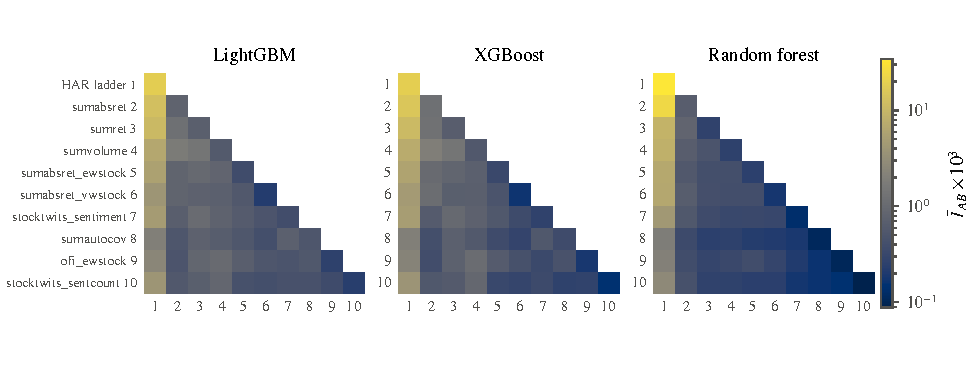
\includegraphics[width=\linewidth]{figures/rehaul_fi_inter_heatmap.pdf}
\caption{The trees' series-level SHAP interactions: $\bar I_{AB}$, the mean over the 1{,}469 scored sessions of $|\phi_{t,AB}|$, $\phi_{t,AB} = \sum_{j\in A}\sum_{l\in B}(\phi_{t,jl} + \phi_{t,lj})$, $\times 10^{3}$, log colour scale shared by the panels; lower triangle, the diagonal is the interaction among a unit's own columns, $\sum_{j \ne l \in A}\phi_{t,jl}$. Units: the 10 with the largest share of their model's off-diagonal interaction mass, summed over the three models; numbered as in the left panel. Local refits on the held-out rows of each of the 147 refits.}
\label{fig:rh_fi_inter}
\end{figure}
